\chapter{Metodología de Trabajo}

\epigraph{Nada se edifica sobre la piedra, todo
sobre la arena, pero nuestro deber es edificar
como si fuera piedra la arena.
}%
{\textbf{Jorge Luis Borges:} \\ \emph{Fragmentos de un evangelio apócrifo}}

\par Los sistemas de software requieren un tiempo y esfuerzo considerable para su desarrollo. Durante este tiempo, desde que se detecta la necesidad de construir un sistema de software, se identifican diferentes etapas que en conjunto se denominan \emph{el ciclo de vida del software}. En cada caso, en función de las características del proyecto, se configurará el ciclo de vida de forma diferente.
\par En particular, \remo se abordó empleando un enfoque metodológico que ordena rigurosamente las diversas etapas de desarrollo denominado \emph{Modelo de Desarrollo en Cascada}. A continuación se detallan algunos aspectos esenciales de dicho modelo y algunas consideraciones. 

\section{Modelo en Cascada}
\par El \emph{Modelo en Cascada Clásico} es un enfoque metodológico secuencial de desarrollo en el que los pasos de desarrollo son vistos hacia abajo (como una ``cascada de agua''), de tal forma que el inicio de cada etapa debe esperar a la finalización de la etapa anterior. La primera descripción formal de este método  fue desarrollada por Winston Royce W. (1929–1995) en 1970, aunque Royce no utiliza el término ``cascada'' en su artículo\cite{royce}. 

\subsection{Etapas del Modelo}
\label{modelo}
A continuación se detallan las diferentes etapas del modelo empleado.

\subsubsection{Elicitación de Requerimientos} 
\par Corresponde al estableciendo de los requisitos de todos los elementos que formarán parte del producto. En esta fase se analizan las necesidades de los usuarios finales del software para determinar qué objetivos debe cubrir. De esta fase surge un documento llamado \textit{``SRS''} (Documento de Especificación de Requisitos), que contiene la especificación completa de lo que debe hacer el sistema sin entrar en detalles internos.

\subsubsection{Análisis de Requerimientos}
\par Consiste en la investigación respecto al dominio de trabajo con el fin de comprender los requisitos de la etapa anterior. Se espera un conjunto de bibliografía y trabajos relacionados, con una breve descripción detallada de ellos (que se utilizará durante el diseño). 	
	
\subsubsection{Diseño}
\par El diseño del software se enfoca en cuatro atributos distintos del programa: la estructura de los datos, la arquitectura del software, el detalle procedimental y la caracterización de la interfaz. El proceso de diseño traduce los requisitos en una representación del software con la calidad requerida antes de que comience la codificación.
\par Como resultado de esta etapa surge el \textit{``SDD''} (Documento de Diseño del Software), que contiene la descripción de la estructura relacional global del sistema y la especificación de lo que debe hacer cada una de sus partes, así como la manera en que se combinan unas con otras.
\par Es conveniente distinguir entre diseño de alto nivel o arquitectónico y diseño detallado o de bajo nivel.

\subsubsection{Codificación}
\par Es la fase en donde se implementa el código fuente, haciendo uso de prototipos así como de pruebas y ensayos para corregir errores.

\subsubsection{Prueba}
\par La prueba se centra en la lógica interna del software, y en las funciones externas, realizando pruebas que aseguren que la entrada definida produce los resultados que realmente se requieren.

\subsection{Ventajas y Desventajas}
\par Luego de estudiar el modelo, se pueden detallar algunas ventajas y desventajas del mismo.
\begin{itemize}
    \item \textbf{Ventajas} 
	    \begin{itemize}    	
	    	\item La planificación es sencilla.
	    	\item Se tiene todo organizado y no se mezclan las fases.
	    	\item Las fases son conocidas por los desarrolladores ya que sigue los pasos intuitivos necesarios a la hora de desarrollar el software.
	    	\item Las etapas y actividades están bien marcadas para facilitar la comprensión y claridad de los objetivos del proyecto.
	    \end{itemize}
	  
	\item \textbf{Desventajas}
		\begin{itemize}
			\item Iteraciones costosas.
			\item El cliente debe tener paciencia. Hasta llegar a las etapas finales del proyecto, no estará disponible una versión operativa del programa. 
			\item Un error importante no detectado hasta que el
            programa este funcionando puede ser desastroso. 
		\end{itemize}
\end{itemize}

\subsection{Consideraciones del Modelo}
\par Para implementar el presente modelo en cascada se tuvieron en cuenta ciertas consideraciones con respecto al contexto en que se desarrollo.

\par Por un lado, las etapas mencionadas en la subsección 3.1.1 fueron llevadas a cabo por una misma persona. En este sentido, se uso el \emph{modelo en cascada con ``solapamiento''}, también conocido como \emph{Sashimo}\cite{Mcconnell96}, que permite comenzar una etapa sin haber terminado por completo la etapa anterior. 

\par Por otro lado, el rol de ``cliente'' en el proceso de desarrollo fue llevado a cabo por miembros de \textbf{FuDePAN} que garantizaron el conocimiento del dominio del problema, no sólo permitiendo realizar la ``Especificación de Requerimientos'' sino que también contaban con los conocimientos técnicos de diseño y programación orientada a objetos como para supervisar el desarrollo. En este sentido, se tomaron algunos elementos de la variante al modelo de cascada “puro” que se conoce como \emph{Staged Delivery}\cite{Mcconnell96} o ``Implementación Incremental'', que permitió realizar revisiones periódicas con miembros de \textbf{FuDePAN} durante las diversas etapas. En la figura~\ref{cascade} se exhibe la estructura clásica del modelo, y las variantes mencionadas.

\begin{figure} [h]
	\hspace*{1cm}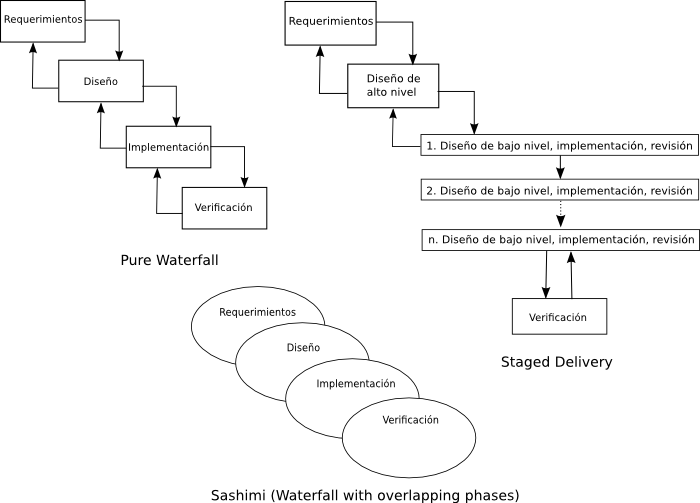
\includegraphics[width=5.2209in,height=3.300in]{image/modelOfCascade.png}
	\caption{Modelos en Cascada [17].}	
	\label{cascade}
\end{figure}

\section{Gestión de la Configuración}
\par Para desarrollar este proyecto fue necesario utilizar un manejador de versiones. Para ello se manipuló un repositorio \emph{Mercurial} (Hg) alojado en GoogleCode\footnote{\url{https://code.google.com/intl/es/}} con el fin de poder seguir la pista a todos los archivos que componen el proyecto.

\section{Prácticas de Software}
\par \remo se desarrolló empleando buenas prácticas de programación las cuales proporcionan múltiples ventajas al desarrollo. Éstas prácticas permiten mantener código limpio, de fácil lectura (sinónimo de fácil mantenimiento), reutilización e integración homogénea, entre otros factores.
A continuación se describen algunos aspectos orientados a \remo:

\begin{itemize}
    \item \textbf{Elicitación y análisis:} aproximadamente el 30 por ciento del tiempo total fue dedicado a éstas etapas, dado que fue necesario investigar el dominio del problema y diversas herramientas a emplear.     

    \item \textbf{Diseño:} se intentó obtener un diseño que respete, entre otras cosas, dos principios básicos: Simplicidad y Ocultamiento de la información. Se utilizaron Patrones de Diseño\cite{Gamma} y UML \\ \cite{uml}.

    \item \textbf{Construcción de código:} aproximadamente el 30 por ciento del tiempo fue dedicado a la construcción del código. Cada vez que se implementó un nuevo componente se chequeó la integración del mismo con todo el proyecto. Cuando superaba la prueba, el código fue trasladado a la rama \emph{default} del repositorio.

    \item \textbf{Revisiones:} la mayoría de las operaciones \emph{commits} realizadas (incluyendo fuente, diagramas, documentos de responsabilidades, entre otros) fueron revisadas por al menos dos personas. No sólo se resaltaron errores, sino también cuestiones en cuando a calidad y eficiencia. Cada vez que se encontró un error o sugerencia, una nueva revisión fue creada conteniendo la solución.

    \item \textbf{Seguimiento de issues:} los bugs y defectos del proyecto fueron reportados como \emph{issues}. Luego, por cada issue, se creo una nueva revisión (rama) conteniendo la solución.
\end{itemize}

\section{Herramientas de Desarrollo Empleadas}
\par Tanto el sistema operativo como todas las herramientas que se usaron para el desarrollo del presente proyecto son libres. \remo tiene la licencia libre \textbf{GPL} (General Public Licence), una copia de la misma pude ser encontrada en \url{http://www.gnu.org/licenses/gpl-3.0.txt}.

\subsection{Lenguaje de Implementación}
\par Como lenguaje de implementación se utilizó \emph{C++}\cite{cplusplus}. 
\par \textit{C++}  es un lenguaje de programación diseñado en el año 1979 por \emph{Bjarne Stroustrup}\footnote{Científico de la computación y catedrático de Ciencias de la Computación en la Universidad A\&M de Texas.} en los laboratorios Bell\footnote{Centros de investigación científica y tecnológica ubicados en más de diez países y que pertenecen a la empresa estadounidense Lucent Technologies.}. En un principio fue una extensión del conocido lenguaje de programación C que fue denominado \emph{``C con clases''}. 

\par El nombre C++ fue propuesto por Rick Mascitti en el año 1983, cuando el lenguaje fue utilizado por primera vez fuera de un laboratorio científico. 

\par En la actualidad, es un lenguaje de tipado estático, multiparadigma, versátil, potente y de propósito general. Su éxito entre los programadores profesionales le ha llevado a ocupar el primer puesto como herramienta de desarrollo de aplicaciones. C++ mantiene las ventajas de C en cuanto a riqueza de operadores y expresiones, flexibilidad, concisión y eficiencia. Además, ha eliminado algunas de las dificultades y limitaciones del C original.

\par Este lenguaje fue elegido porque permite el uso de técnicas orientadas a objetos y produce eficiente código assembly. Además ofrece una gran cantidad de librerías para facilitar la resolución de determinados problemas, permitiendo concentrarse en los mismos y no en implementar tipos de datos abstractos ya conocidos.

\subsection{GNU}
\begin{itemize}
	\item \textbf{GCC (GNU Compiler Collection)\footnote{\url{http://gcc.gnu.org/}}:} conjunto de compiladores creados por el proyecto GNU.
     \textsc{GCC} es software libre y se distribuye bajo licencia \textsc{GPL}. Estos compiladores se
     consideran estándar para sistemas operativos derivados de GNU.

	\item \textbf{GDB (The GNU Project Debbuger)\footnote{\url{www.gnu.org/software/gdb/}}}: es un depurador portable que se puede utilizar en varias plataformas Unix y funciona para varios lenguajes de programación como C y C++ entre otros. \textsc{GDB} fue escrito por Richard 
    Stallman\footnote{Nacido en Manhattan, Nueva York, 16 de marzo de 1953. Fundador del movimiento por el software libre en el mundo.} en 1988, es software libre y se distribuye bajo licencia GPL. 
\end{itemize}	
	
\subsection{Sistema de Construcción}
Para la compilación e inclusión de librería externas, se usó \emph{fudepan-build}\footnote{\url{https://code.google.com/p/fudepan-build/}}, un proyecto de \textbf{FuDePAN} que utiliza scons\footnote{\url{http://www.scons.org/}}.

\subsection{\LaTeX}
\par Esta herramienta fue utilizada para llevar adelante el presente documento y todo la documentación de \textbf{Remo}. Básicamente \LaTeX{}\cite{latex} es un paquete de macros para TEX\footnote{Sistema de composición de textos de alta calidad creado por Donald E. Knuth a finales de la década de los 70, dirigido particularmente a aquellos textos que contienen una gran cantidad de expresiones matemáticas.}, originalmente escrito por Leslie Lamport para proporcionar un sistema de procesamiento de documentos más simple de uso que TEX, pero con toda su potencia. 
\par El formato de los archivos es mucho más estable que en otros procesadores de texto, cualquier cambio es realizado localmente y no repercute en efectos colaterales, existen implementaciones para distintas plataformas y en todas el resultado es exactamente el mismo (si se tienen los mismos estilos y tipos). 

\subsection{Edición}
\begin{itemize}
	\item \emph{Gedit\footnote{\url{http://projects.gnome.org/gedit/}}:} para la edición de texto plano.   
    \item \emph{Sublime\footnote{\url{www.sublimetext.com}}:} para la edición de texto plano. Permite simular un excelente IDE de desarrollo.
\end{itemize}

\subsection{Gráficos}
\begin{itemize}
	\item \emph{Gimp\footnote{\url{www.gimp.org}}:} editor de imágenes.
	\item \emph{Bouml\footnote{\url{http://www.bouml.fr/}}:} editor de diagramas UML.
	\item \emph{Dia\footnote{\url{http://live.gnome.org/Dia}}:} editor de diagramas de propósito general.
    \item \emph{Diagramas online\footnote{\url{www.websequencediagrams.com}}:} editor de diagramas de secuencia.
\end{itemize}

\subsection{Análisis Estático de Código}
\begin{itemize}
 \item \emph{Astyle}\footnote{\url{http://astyle.sourceforge.net}}: indentador de código fuente, formateador y embellecedor para los lenguajes C, C++, C\# y Java.

 \item \emph{cppcheck\footnote{\url{http://sourceforge.net/apps/mediawiki/cppcheck}}:} permite detectar los tipos de errores que los compiladores normalmente no detectan. El objetivo es detectar sólo los errores reales en el código (es decir, ningún falsos positivos).

\item \emph{Cloc\footnote{\url{http://cloc.sourceforge.net/}}:} es un programa para contar la cantidad de lineas del sistema.

\item \emph{CCCC\footnote{\url{http://cccc.sourceforge.net/}}:} herramienta que analiza los fuentes y genera reportes en varias métricas asociadas al código.

\item \emph{GCov\footnote{http://gcc.gnu.org/onlinedocs/gcc/Gcov.html}:} es una herramienta GNU para realizar pruebas de cobertura sobre código fuente. Se utiliza en conjunto con \textbf{\textit{gcc}} para determinar el número de veces que cada línea de un programa se ejecuta durante una ejecución. Esto hace que sea posible encontrar áreas del código que no se utilizan, o que no se ejecutan en los casos de pruebas  planteados.

\end{itemize}

\subsection{Análisis Dinámico de Código}
\begin{itemize}
	\item Valgrind\footnote{\url{http://valgrind.org}}: permite el análisis dinámico de código. Puede detectar automáticamente \emph{memory leaks} y errores de contexto.
\end{itemize}

\subsection{Automatización de Pruebas}
Se empleó gtest\footnote{\url{http://googletest.googlecode.com}} y gmock\footnote{\url{http://googlemock.googlecode.}} para la elaboración y ejecución de pruebas.